\documentclass[crop,tikz]{standalone}% 'crop' is the default for v1.0, before it was 'preview'
%\usetikzlibrary{...}% tikz package already loaded by 'tikz' option
\usepackage{color}
\newcommand{\gv}[1]{\ensuremath{\mbox{\boldmath$ #1 $}}} 
\renewcommand{\v}[1]{\ensuremath{\mathbf{#1}}}
\newcommand{\name}[1]{_{\text{#1}}}
\usepackage{siunitx}

\begin{document}
 \begin{tikzpicture}
    %Lipid molecule
    \node[label={[yshift=0cm,xshift=1.7cm]\textbf{Standard model for DPPC:}}](dppc) at (-0.25,0) {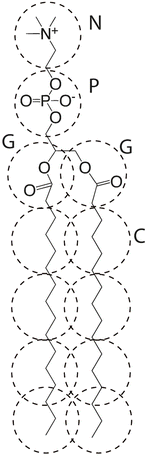
\includegraphics[width=0.125\textwidth]{DPPC_REP.png}};

    %\node(standard) at (1,3){The standard model:};
    %Equations
    \node[anchor=west] (eq1) at (0.6,2.){\( H_0=\sum\frac {m_iv_i^2}2\v  +\sum\frac {k_r(r_{ij}-r_0)^2}2+\sum\frac {k_\theta(\cos(\theta_{ijk})-\cos(\theta_{0}))^2}2\)};    
    \node[anchor=west] (eq2) at (0.6,1.){\( W_0=\frac 1{2\rho_0}\int\text d \v r~(\sum_{k\ell}\textcolor{red}{\tilde\chi_{k\ell}}\phi_k(\v r)\phi_\ell(\v r)+\frac{1}\kappa\left(\sum_\ell\phi_\ell(\v r)-a\right)^2)\)};

    %Kst
    \node[](chi) at (6,-1){\scriptsize
      \begin{minipage}{0.4\textwidth}
        \begin{tabular}{cccc|r}
          \hline\hline
          G& P& C &W&\\
          \hline
          -1.50   &  6.30  &   9.00 &    -8.10&N\\
          & 4.50  &  13.50 &    -3.60&P\\
          &  &  6.30  &    4.50 &G\\                                                                                                                                 
          &  &   &    33.75&C\\
        \hline\hline
        \end{tabular}
      \end{minipage}
    };%label={[yshift=-2cm,xshift=-1cm]$\textcolor{red}{\tilde \chi_{k\ell$}} /\si{kJ.mol^{-1}}}
    \node (d) at ([xshift=1.1cm,yshift=.5cm]chi.south west){$\textcolor{red}{\tilde\chi_{k\ell}} /{\footnotesize \si{kJ.mol^{-1}}}$};
    %\draw ([yshift=0.25cm,xshift=0.3cm]chi.south)--([yshift=0.35cm,xshift=0.1cm]chi.west);

    \node[anchor=west] (eq3) at (-1.,-3){\textbf{Modeling of tension:} \( W_1=-\frac 1{\rho_0}\int\text d \v r~\left(\textcolor{blue}{K\name{ST}} \gv\nabla\phi\name{W}(\v r)\cdot\gv\nabla\phi\name{C}(\v r)\right)\)};
    %   \node(kst) at (5,-1.5){Water-carbon-interaction: $\textcolor{blue}{K\name{{ST}}}\equiv-K\name{{CW}}$};
    %% \node[anchor=west](kst1) at(3,-4.) {$\textcolor{blue}{K\name{ST}}<0$: \textit{Energy \textbf{loss} for surface area}};
    %% \node[anchor=west](kst1) at(3,-4.5){$\textcolor{blue}{K\name{ST}}>0$: \textit{Energy \textbf{gain} for surface area}};
  

  \end{tikzpicture}
\end{document}
